% !TEX encoding = UTF-8
% !TEX TS-program = pdflatex
% !TEX root = ../Appunti.tex

In questo capitolo viene affrontato il tema dei solidi. Questa affermazioni però apre uno spettro fin troppo ampio in confronto agli argomenti che verranno trattati, nei quali si discuterà delle proprietà dovute a un qualche tipo di reticolo cristallino.

Da qui il nome del capitolo.

\section{Il dilemma della capacità termica}

La spiegazione dell'andamento con la temperatura della capacità termica dei solidi, illustrata in \cref{fig:heatcap}, è uno dei successi della teoria quantistica, ottenuto già nell'ambito della \textit{old quantum theory}.

\begin{figure}[h]
	\centering
	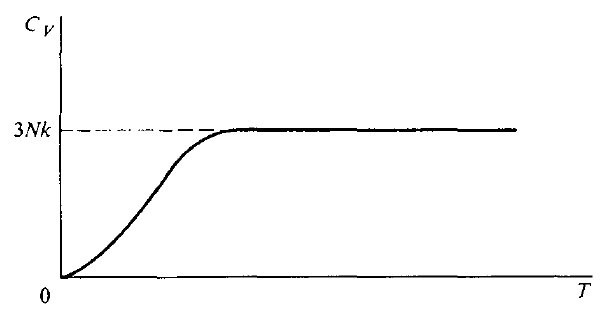
\includegraphics[width=0.6\textwidth]{Immagini/HeatCapacity.png}
	\vspace{-10pt}
	\caption{}
	\label{fig:heatcap}
\end{figure}

Si procederà esponendo i vari passaggi dell'evoluzione della teoria che sono stati compiuti storicamente: il teorema di equipartizione, il modello di Einstein e infine quello di Debye.

\subsection{Teorema di equipartizione}

Per studiare il comportamento degli atomi in un reticolo cristallino si introduce innanzi tutto l'\textit{approssimazione di campo medio}.

\begin{defn}[Campo medio]
	Si chiama \textit{approssimazione di campo medio} (o \textit{teoria}) un metodo che prevede di considerare, anziché per ogni particella le interazioni con ogni altra particella del sistema, solo un contributo mediato su tutte le altre particelle e incluso nella forma di un potenziale esterno in cui si trovi la singola particella in esame. 
\end{defn}

Nel caso in esame si considererà per ogni atomo del reticolo un potenziale efficace che lega il singolo atomo alla sua posizione di equilibrio.
Sia quindi $ \textbf{r} $ il vettore che indica lo spostamento dalla posizione di equilibrio, e $ u $ il potenziale efficace.
Poichè nella posizione di equilibrio non ci sono forze non bilanciate allora:
\begin{equation*}
	\partdev{u}{\textbf{\textbf{r}}} = 0	\qquad	\partdev{^2 u}{\textbf{\textbf{r}}^2} > 0
\end{equation*}
per cui si può espandere il potenziale efficace nel modo seguente:
\begin{equation*}
	u = u_0 + \frac{\alpha}{2} \textbf{r}^2
\end{equation*}
con $ \alpha = (\partial^2 u / \partial \textbf{r}^2)_{r=0} > 0 $. Con $ u_0 $ negativo, perché è l'energia di legame degli atomi ai siti dl reticolo.

Da tale potenziale si ottiene la legge di dispersione:
\begin{equation*}
	\varepsilon(\textbf{r}, \textbf{p}) = u_0 + \frac{\textbf{p}^2}{2m} + \frac{\alpha\textbf{r}^2}{2}
\end{equation*}

Per cui si ottiene per la funzione di partizione di singola particella:
\begin{align*}
	Z_1 &= \frac{1}{(\hplanck)^3} \int \cdots \int \exp[-\frac{\varepsilon(\textbf{p},\textbf{r})}{\kt}] \dd^3 p ~\dd^3 r =\\
	&= \frac{\exp(-u_0/\kt)}{(\hplanck)^3} \left[\int \exp(- \frac{p^2}{2 m \kt})\dd p\right]^3\left[\int \exp(- \frac{\alpha x^2}{2 \kt}) \dd x\right]^3
\end{align*}
Coefficienti a parte i due integrali che compaiono nell'espressione precedente sono identici:
\begin{equation*}
\int \exp(- \frac{a \xi^2}{\kt}) \dd xi = \frac{1}{2} \left(\frac{\kt}{a}\right)^{1/2} \int \eta^{1/2} e^{-\eta} \dd \eta
\end{equation*}

Riguardo i limiti di integrazione si nota che mentre per gli impulsi sono possibili tutti i numeri reali, per le posizioni ci si dovrebbe limitare ad una piccola area attorno alla posizione di equlibrio, che è quella in cui si è effettuato lo sviluppo.

Questo non è strettamente rilevante, infatti l'esponenziale si smorza fortemente anche per spostamenti non troppo grandi, per cui si può integrare anche qui da $ - \infty $ a $ + \infty $.

Si ha quindi per $ Z_1 $:
\begin{equation*}
	Z_1 = A (\kt)^3 \exp(-\frac{u_0}{\kt})
\end{equation*}
con $ A $ una costante (in cui è inclusa fra le altre cose la sesta potenza di $ \int_{0}^{\infty} \eta^{1/2} e^{-\eta} \dd \eta $).

Nonostante le considerazioni fatte nella \cref{sec:idpart} riguardo alle particelle identiche, qui non si hanno effetti di questo tipo poiché le particelle possono essere distinte in base al sito del reticolo che occupano. Per cui:
\begin{equation*}
Z = Z_1^N = A^N (\kt)^{3N} \exp(-\frac{N u_0}{\kt})
\end{equation*}
da cui si ricava l'energia libera:
\begin{equation*}
F = - \kt \log Z = N u_0 -3 N \kt \log\kt - N\kt \log A
\end{equation*}
e quindi l'entropia:
\begin{equation*}
S = - \partfix{F}{T}{V,N} = 3 N k_B \log\kt + 3 N k_B - N k_B \log A
\end{equation*}
e infine la capacità termica e l'energia:
\begin{align*}
C_V &= T \partfix{S}{T}{V,N} = 3 N k_B\\
E &= F + TS = 3 N \kt + N u_0
\end{align*}

I risultati ottenuti sono molto semplici e altrettanto chiari: l'energia è data dalla somma delle energie di legame di tutti gli atomi più il contributo termico per tutti i gradi di libertà.\footnote{La capacità termica trovata è nota come \textit{legge di Dulong-Petit.}}

Allo stesso modo la capacità termica è la somma dei contributi dei vari gradi libertà, $ 6 $ per ogni particella: $ 3 $ traslazionali e $ 3 $ vibrazionali. Il fatto più rilevante è che questo contributo sia pari a $ \frac{1}{2} k_B$ per ogni grado di libertà, indipendentemente dalla tipologia e dai dettagli del modello, per cui le costanti non entrano in gioco.

Questo è il contenuto del \textit{teorema di equipartizione}.

\begin{es}[Gas ideale]
	Nel modello di gas ideale i gradi di libertà erano solo 3, quelli traslazionali, e infatti la capacità termi trovata era $ \frac{3}{2} N k_B$.
\end{es}

Questo risultato è in accordo con i dati sperimentali ad alte temperature, ma non descrive l'andamento mostrato on \cref{fig:heatcap} per basse $ T $.

\subsection{Modello di Einstein}
\label{sec:einheatcap}

Il modello di Einstein è anch'esso una teoria di campo medio, in cui si considera un insieme di $ 3N $ oscillatori armonici indipendenti, esattamente come nel caso precedente.

L'unica differenza nelle ipotesi di partenza è nell'introduzione di un concetto quantistico: la \textit{quantizzazione dei livelli energetici} del singolo oscillatore.
\newline

Quanto scritto sopra si traduce in una enumerazione delle possibili energie del singolo oscillatore armonico:
\begin{align*}
	\varepsilon_\omega &= (n + 1/2) \hbar \omega + u_0/3 = \varepsilon_{0 \omega} + n \hbar \omega\\
	con &\qquad \varepsilon_{0 \omega} =  \frac{\hbar \omega}{2}  + \frac{u_0}{3}
\end{align*}
dove $  \varepsilon_{0 \omega} $ è l'energia del fondamentale. Come nel paragrafo precedente la frequenza è la stessa per tutti gli oscillatori.

La funzione di partizione del singolo oscillatore è:
\begin{equation*}
	Z_{1\omega} = \exp(-\frac{ \varepsilon_{0 \omega}}{\kt}) \sum_n \left[\exp(-\frac{ \hbar \omega}{\kt})\right]^n = \frac{\exp(- \varepsilon_{0 \omega}/\kt)}{1 - \exp(- \hbar \omega/\kt)}
\end{equation*}

Poiché i $ 3N $ oscillatori armonici sono tutti identici e indipendenti è sufficiente trovare le proprietà termodinamiche di singolo oscillatore, le altre si ottengono per estensività:
\begin{align*}
	F_{1\omega} &= - \kt \log Z_{1\omega}  = \varepsilon_{0 \omega} + \kt \log \left[1 - \exp(-\frac{ \hbar \omega}{\kt})\right]\\
	S_{1\omega} &= - k_B \log \left[1 - \exp(-\frac{ \hbar \omega}{\kt})\right]  + \frac{\hbar \omega}{T} \frac{\exp(- \hbar \omega/\kt)}{1 - \exp(- \hbar \omega/\kt)}\\
	E_{1\omega} &= 	F_{1\omega} + T S_{1\omega} = \varepsilon_{0 \omega} + \bar{n} \hbar \omega\\
	\bar{n} &= \frac{\exp(- \hbar \omega/\kt)}{1 - \exp(- \hbar \omega/\kt)} = \frac{1}{\exp(\hbar \omega/\kt) - 1}
\end{align*}
si noti che $ \bar{n} $ coincide con il numero di occupazione medio di ogni stato di singola particella di un gas di Bose degenere ($ \mu = 0 $); questa corrispondenza non è casuale.

Quindi per valutare le proprietà termodinamiche dell'intero sistema si moltiplicano per $ 3N $ quelle trovate per il singolo oscillatore. In particolare, per la capacità termica:
\begin{equation*}
	C_V = \partfix{E}{T}{V} = 3N \partfix{E_{1\omega}}{T}{V} = 3 N k_B \left(\frac{\hbar \omega_E}{\kt}\right)^2 \frac{\exp(\hbar \omega_E/\kt)}{[\exp( \hbar \omega_E/\kt) - 1]^2}
\end{equation*}
dove si è indicata con $ \omega_E $ la frequenza propria degli oscillatori, che sarà una proprietà del materiale. Si definisce frequentemente la temperatura di Einstein $ \Theta_E $:
\begin{equation*}
	k_B \Theta_E = \hbar \omega_E
\end{equation*}
in termini della quale si può riscrivere l'espressione della capacità termica.

Ad alte temperature, $ T \gg \Theta_E $, si ha per la capacità termica, approssimando al primo ordine:
\begin{equation*}
	C_V \rightarrow 3N k_B
\end{equation*}
cioè il risultato classico.
Nel limite opposto si ottiene invece:
\begin{equation*}
C_V \rightarrow 3N k_B \left(\frac{\hbar \omega_E}{\kt}\right)^2 \exp(-\frac{\hbar \omega_E}{\kt})
\end{equation*}
cioè che $ C_V \rightarrow_{T \rightarrow 0} ~0 $, che è in accordo con quanto mostrato in \cref{fig:heatcap}.

Questo risultato poteva essere previsto dalla meccanica quantistica: a temperatura $ T \rightarrow 0 $ il sistema si trova nel fondamentale, e la probabilità di eccitazione va a $ 0 $ con la temperatura, poiché $ \partial S / \partial T $ è finito.
\newline

Il modello di Einstein presenta un paio di incongruenze rispetto alle proprietà di un cristallo reale:
\begin{itemize}
	\item La capacità termica si annulla troppo rapidamente per $ T \rightarrow 0 $, infatti in questo limite si trova sperimentalmente:
	\begin{equation*}
	C_V \propto T^3
	\end{equation*}
	
	Il fatto che il modello di Einstein presenti un andamento esponenziale è dovuto alla struttura dei livelli energetici, in particolare alla presenza di un \textit{gap} finito tra il fondamentale e il primo eccitato.
	A causa di questa separazione se l'energia termica a disposizione diminuisce la probabilità di eccitazione decresce esponenzialmente, e quindi anche la capacità termica.
	\item L'altro problema è dato dai parametri del materiale $ u_0, \omega_E $. In una teoria di campo medio consistente queste quantità non possono dipendere dalla spaziatura tra gli atomi, poiché se così fosse il moto di un atomo influenzerebbe il vicino ed essi non sarebbero indipendenti.
	
	La spaziatura tra gli atomi non è altro che l'inverso della densità, e la richiesta che i parametri non dipendano dalla densità, e quindi dal volume se il numero di particelle è fissato, implica che:
	\begin{equation*}
		P = - \partfix{F}{V}{T,N} = 0
	\end{equation*}
	poiché la $ F $ dipende solo dalla $ F $ di singolo oscillatore, che contiene solo l'informazione sui parametri, e dal numero di oscillatori presenti.
	
	Analogamente la compressibilità isoterma diverge:
	\begin{equation*}
	K_T = - \frac{1}{V} \partfix{V}{P}{T,N} = - \left[V \partfix{^2 F}{V^2}{T,N}\right]^{-1}
	\end{equation*}	
\end{itemize}

Ovviamente in un cristallo reale il potenziale su un atomo dipende dalla posizione dei vicini, e quindi non sono indipendenti. La cosa inattesa è che migliorando il modello per risolvere il secondo punto anche il comportamento della capacità termica diventa quello corretto.

Si consideri un cristallo a temperatura nulla: esso sarà nel fondamentale e i suoi atomi saranno disposti in un reticolo regolare per minimizzare l'energia.
Non appena si inserisce un minimo di energia nel sistema, aumentando così la temperatura, ogni possibile tipo di eccitazione ne acquisirà una parte proporzionale a $ e^{-\mathcal{E}/\kt} $, dove $ \mathcal{E} $ è l'energia dell'eccitazione, e quindi ognuna contribuirà alla capacità termica con un termine proporzionale a $ e^{-\mathcal{E}/\kt} $. Per cui più piccola sarà $ \mathcal{E} $, più grande sarà il contributo alla capacità termica.

Si cerca quindi di costruire il primo livello eccitato del sistema, che sarà quello che maggiormente contribuirà alla capacità termica.

Si immagini di spostare un atomo dalla sua posizione di equlibrio: questo aumenterà la sua energia e quella dei suoi vicini. Per ottenere una configurazione a energia più bassa si può pensare di spostare anche i vicini in modo solidale, e quindi i loro vicini, \dots.
Se si estende questo procedimento a tutto il cristallo si è semplicemente spostato il suo centro di massa, senza modificare le posizioni relative, e quindi l'energia del sistema (in assenza di campi esterni ci sarà invarianza per traslazioni globali).

Per ottenere un risultato significativo anziché spostare solidalmente ogni atomo e i suoi vicini si può applicare ai vicini uno spostamento coerente, ma leggermente ridotto, in modo che le distanze relative cambino poco fra primi vicini.
Più esplicitamente, si pensi a un cristallo unidimensionale finito: si tengono fermi gli estremi, e partendo da uno dei due si aumenta gradualmente lo spostamento di ogni atomo dalla sua posizione di equilibrio, per poi diminuirlo  non appena superata la metà.

In questo modo si ottengono le onde sonore nei cristalli.
\newline

Dal risultato ottenuto si evince che la capacità termica a bassa temperatura è dominata dai modi collettivi del sistema, piuttosto che da quelli incoerenti come nel caso del modello di Einstein.

Si possono pensare questi modi organizzati come nel caso del modello di Einstein: un insieme di $ 3N $ oscillatori indipendenti, ciò che differisce dal caso precedente è che la frequenza non è unica, ma dipende dal modo considerato.

\begin{defn}[Modi normali]
	I modi collettivi descritti sono detti \textit{modi normali} e sono quelli che diagonalizzano l'Hamiltoniano del sistema (proprio per questo sono indipendenti).
\end{defn}

Le proprietà termodinamiche saranno quindi saranno calcolate in modo simile a quelle del modello di Einstein, ma per ottenere il risultato sarà necessario conoscere la distribuzione in frequenza dei modi normali.
\begin{align*}
	F &= E_0 + \kt \sum_\alpha \log \left[1 - \exp(-\frac{\hbar \omega_\alpha}{\kt})\right]\\
	E &= E_0 + \sum_{\alpha} \bar{n}_\alpha \hbar \omega_\alpha\\
	\text{con}	&\qquad  \bar{n}_\alpha = \frac{1}{\exp(\bar{n}_\alpha/\kt) - 1}
\end{align*}

\subsubsection{Numero di modi normali}

Il modo più corretto per capire quanti modi normali ci siano è esaminare la struttura delle equazioni, e si ottiene facilmente che se le equazioni in campo medio hanno $ 3N $ soluzioni, corrispondenti al numero di oscillazioni indipendenti, allora modificando le equazioni si otterrano soluzioni più complicate, ma il numero sarà sempre lo stesso per i teoremi generali sulla teoria delle equazioni differenziali lineari.
\newline

C'è un altro modo però per ottenere tale numero nel caso del modello considerato, esaminando il limite per alte $ T $, cioè il limite classico.

In tale limite il sistema soddisfa le ipotesi del teorema di equipartizione, e quindi studiando il valore dell'energia:
\begin{align*}
 \bar{n}_\alpha &\simeq \frac{\kt}{\hbar \omega_\alpha} \implies  \bar{n}_\alpha \hbar \omega_\alpha \simeq \kt \implies \\
 &\implies E \simeq E_0 + \tilde{N} \kt
\end{align*}
è lo stesso teorema di equipartizione a imporre $ \tilde{N} = 3N  $, dove $ \tilde{N} $ è il numero di modi normali.

\subsection{Modello di Debye}

Quanto detto nella \cref{sec:einheatcap} a proposito delle onde sonore è alla base del modello di Debye. Si procederà quindi ricavando prima la legge di dispersione per basse frequenze, in modo da poter determinare il comportamento a bassa temperatura della capacità termica.

\subsubsection{Legge di dispersione per onde lunghe}

Nei cristalli le onde sonore hanno $ 3 $ polarizzazioni, due trasverse e una longitudinale, cui corrispondono anche due diverse velocità $ c_t $ e $ c_l $.
Per semplificare la trattazione si considererà solamente quella longitudinale.
Il risultato ottenuto sarà comunque applicabile esattamente per i liquidi\footnote{Essi non hanno polarizzazioni trasverse, perché gli strati scorrono l'uno sull'altro.}.
\newline

\noindent Poiché si sta cercando il comportamento delle onde lunghe si può trascurare la struttura atomica, e considerare il mezzo come un continuo.

Dalla legge di Newton si ricava:
\begin{equation*}
\partdev{P}{x} + \rho\partdev{v}{t} = 0
\end{equation*}
mentre dalla conservazione della massa:
\begin{equation*}
\partdev{\rho}{t} + \partdev{\rho v}{x} = 0
\end{equation*}
dove in entrambe $ \rho $ è la densità, $ P $ la pressione, $ t $ il tempo, $ x $ la coordinata spaziale e $ v $ la velocità.

Poiché si cerca il comportamento per piccoli spostamenti dalle posizioni di equilibrio è utile definire le equazioni proprio in termini di queste variazioni:
\begin{align*}
P &= P_0 + P'\\
\rho &= \rho_0 + \rho'\\
v &= v'
\end{align*}
e scrivendo le equazioni al prim'ordine in questi spostamenti (cioè eliminando i termini in cui compaiono più di un fattore primao):
\begin{equation*}
\begin{cases*}
\partdev{P'}{x} + \rho_0 \partdev{v'}{t} = 0\\
\partdev{\rho'}{t} + \rho_0 \partdev{v'}{x} = 0
\end{cases*}
\end{equation*}

Si hanno perciò tre incognite e due equazioni. Per risolvere questo problema si considera quindi che la densità sia una funzione della sola pressione $ \rho \equiv \rho(P) $, e di conseguenza:
\begin{equation*}
\rho = \rho(P_0) + \partdev{\rho}{P} P' \qquad \implies \qquad \rho' = \partdev{\rho}{P} P' = \frac{1}{c^2} P'
\end{equation*}
dove si è definito\footnotemark:
\footnotetext{Si ha infatti:
	\begin{equation*}
	\partfix{\rho}{P}{N,T/S} = \partfix{N/V}{P}{N,T/S} = - \frac{N}{V^2} \partfix{V}{P}{N,T/S} = \rho K_{T/S}
	\end{equation*}
}
\begin{equation*}
c^2 = \partdev{P}{\rho} = \frac{1}{K \rho}
\end{equation*}
Nell'equazione di stato la densità dipende sia dalla pressione che dalla temperatura. ignorare la dipendenza dalla temperatura corrisponde a ignorare la differenza tra $ C_P $ e $ C_V $, o tra $ K_T $ e $ K_S $, che è una buona approssimazione per i mezzi continui, dove le compressibilità sono piccole\footnote{Nella \cref{sec:thermdev} si è trovato infatti che la differenza delle capacità termiche è proporzionale al quadrato di $ (\partial V / \partial T)_P $.}. Perciò il $ K $ che appare nell'espressione precedente è indifferente quale sia.

Si ottengono quindi le equazioni:
\begin{equation*}
\begin{cases*}
c^2\partdev{\rho'}{x} + \rho_0 \partdev{v'}{t} = 0\\
\partdev{\rho'}{t} + \rho_0 \partdev{v'}{x} = 0
\end{cases*}
\end{equation*}
e prendendo $ \partial/\partial x $ della prima e $ \partial/\partial t $ della seconda e sottraendo si ha:
\begin{equation*}
	\partdev{^2\rho}{x^2} - \frac{1}{c^2} \partdev{^2\rho}{t^2} = 0
\end{equation*}
che è la nota equazione di D'Alembert che ammettono soluzioni propaganti con una legge di dispersione lineare.
\begin{equation*}
	\omega = \pm c q
\end{equation*}

Si ottiene infine che $ \omega $ assume un insieme di valori discreto, determinato dall'insieme di valori discreto che può assumere $ q $, fissando, ad esempio, condizioni periodiche al contorno:
\begin{equation*}
	\rho'(x=0) = \rho'(x=L)
\end{equation*}
che implicano per $ q $:
\begin{equation*}
	q = \frac{2\pi}{L}n
\end{equation*}
dove $ n $ è un numero intero, limitato dall'alto (se avessimo la legge di dispersione esatta il limite sarebbe fissato dal passo reticolare, ma poiché si sta trattando il caso di onde lunghe il limite è fissato dagli estremi di validità  dell'approssimazione).

\subsubsection{Capacità termica e proprietà termodinamiche}

Si applica quindi il risultato trovato per la legge di dispersione, distinguendo però le tre polarizzazioni. Per farlo si indica la generica velocità con $ c_i $, $ i = l,t $.
\newline

Poiché il numero di modi per ogni polarizzazione è molto grande, dell'ordine di $ N $, le somme possono essere convertite in integrali, per cui anche l'enumerazione dei modi va trasformata in una densità di modi.

Per l'enumerazione si aveva:
\begin{align*}
	\textbf{q} &= \left(\frac{2\pi}{L}\right) \textbf{n}\\
	\text{con} &\qquad \textbf{n} = n_1 \hat{\textbf{x}} + n_2 \hat{\textbf{y}} + n_3 \hat{\textbf{z}}
\end{align*}
e poiché il cristallo immaginato ha dimensione $ L $ per ogni lato si ha $ V = L^3 $. Il numero di modi compreso tra $ \textbf{n} $ e $ \textbf{n} + \dd \textbf{n} $, cioè $ \dd \textbf{n} $, è quindi un differenziale tridimensionale $ \dd \textbf{n} = \dd^3 n $.

Il numero di modi compresi tra $ \textbf{q} $ e $ \textbf{q} + \dd \textbf{q} $ è:
\begin{align*}
	\dd^3 n &= \frac{V}{(2\pi)^3} \dd^3 q \implies\\
	&\implies \dd^3 n = \frac{4\pi V q^2 \dd q}{(2\pi)^3}
\end{align*}
in cui nella seconda si è assunto che il solido sia isotropo.

Dalla legge di dispersione si ottiene infine:
\begin{equation*}
	\rho_i(\omega) \dd \omega = \frac{4\pi V}{(2\pi)^3} q(\omega)^2 \dd q(\omega) = \frac{4\pi V}{(2\pi c_i)^3} \omega^2 \dd \omega
\end{equation*}
La densità di modi ha lo stesso ruolo che la densità di stati di singola particella aveva nel \cref{chap:gas}. La differenza principale tra i due casi sta proprio nella legge di dispersione, che implica una diversa densità, esattamente come si era trovato nell'\cref{es:lindisp}.

Inoltre il ruolo del numero di particelle nello stato (numero di occupazione) è qui assunto dal numero di eccitazioni di un certo oscillatore.

Tutte queste analogie portano a definire l'eccitazione elementare come una particella, o meglio una \textit{quasiparticella} (vedi \cref{sec:idpart}), e trattare l'insieme degli oscillatori come un gas perfetto di eccitazioni non interagenti: nei cristalli sono dette \textit{fononi}.
\newline

Se il cristallo è isotropo le due polarizzazioni trasverse hanno la stessa velocità di propagazione, e sommando sulle tre polarizzazioni si ottiene:

\begin{equation*}
\rho(\omega) \dd \omega = \frac{4\pi V}{(2\pi)^3}\left(\frac{1}{c_l^3} + \frac{2}{c_t^3}\right) \omega^2 \dd \omega
\end{equation*}
e definendo:
\begin{equation*}
	\frac{3}{\tilde{c}^3} = \frac{1}{c_l^3} + \frac{2}{c_t^3}
\end{equation*}
si ha:
\begin{equation*}
\rho(\omega)= \frac{12\pi V}{(2\pi\tilde{c})^3}\omega^2 
\end{equation*}

La formula trovata è stata ricavata assumendo la legge di dispersione per onde lunghe, quindi è valida solo nel limite di bassa frequenze, ma a bassa temperatura, cioè se $ \omega $ è abbastanza grande tale che:
\begin{equation*}
\hbar \omega \gg \kt
\end{equation*}
allora è il numero di eccitazioni a essere esponenzialmente smorzato (vedi \cref{sec:einheatcap}), per cui anche estendendo l'integrale fino a $ \infty $ si commette un errore piccolo.

Si ha quindi per l'energia:
\begin{align*}
	E_{th} = \int_{0}^{\infty} \bar{n}(\omega)\rho(\omega) \hbar \omega \dd \omega = \frac{12\pi V}{(2\pi\tilde{c})^3}\hbar \int_{0}^{\infty} \frac{\omega^3 \dd \omega}{\exp(\hbar\omega/\kt)-1} = \frac{12\pi V}{(2\pi\hbar\tilde{c})^3} (\kt)^4 \int_{0}^{\infty} \frac{x^3 \dd x}{e^x -1}
\end{align*}
L'integrale definito può essere valutato e risulta essere pari a $ \pi^4 / 15 $.

La cosa più importante è che la dipendenza dell'energia è $ E \propto T^4 $ e di conseguenza $ C_V = \partfix{E}{T}{V} \propto T^3$, cioè l'andamento sperimentalmente verificato.
\newline

Si sono trascurati del tutto i modi ad alta frequenza, per cui non è stata neanche trovata la legge di dispersione. Essi però non contribuiscono sostanzialmente in nessuno dei due limiti: per basse temperature sono i coinvolti solo i modi a bassa frequenza, perché quelli ad alta frequenza sono congelati, mentre per temperature alte il teorema di equipartizione impone che l'unica informazione rilevante sia il numero di modi.

Per questo è naturale raccordare i due andamenti semplicemente estendendo il limite di validità della densità di modi e considerando $ \rho(\omega) \propto \omega^2 $ fino a una certa frequenza massima $ \omega_m $ fissata da:
\begin{equation*}
	3N = \int_0^{\omega_m} \rho(\omega) \dd \omega
\end{equation*}
tale interpolazione è proprio ciò che viene chiamato \textit{modello di Debye}.

La frequenza massima $ \omega_m $ è come $ \omega_E $ nel modello di Einstein una proprietà del materiale, e può essere espresso per mezzo della velocità media di propagazione del suono e della densità del materiale:
\begin{equation*}
	\omega_m = 2 \pi \tilde{c} \left(\frac{3N}{4\pi V}\right)^{1/3}
\end{equation*}

Si sarebbe potuto decidere di porre il cutoff in un altro modo, ad esempio facendolo in modo ditinto per ogni polarizzazione, che va pure bene, ma a questo livello è una complicazione non necessaria.

Come nel caso di Einstein anche qui si può definire una temperatura caratteristica, detta \textit{temperatura di Debye} $ \Theta_D $:
\begin{equation*}
\hbar \omega_m = k_B \Theta_D
\end{equation*}
e riportando in un grafico (come in \cref{fig:heatcapdeb}) $ C_V/N k_B $ contro $ T/\Theta_D $ si otttiene un andamento universale, coerente con i dati sperimentali, contrariamente alla \cref{fig:heatcap}.
\newline

\begin{figure}[h]
	\centering
	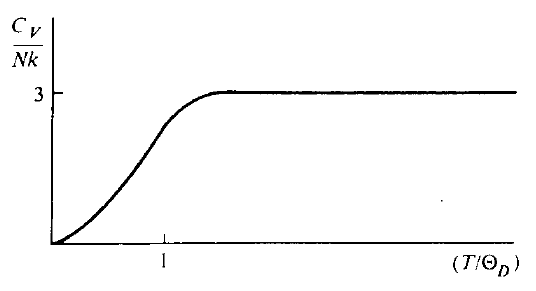
\includegraphics[width=0.6\textwidth]{Immagini/HeatCapacityDebye.png}
	\vspace{-10pt}
	\caption{}
	\label{fig:heatcapdeb}
\end{figure}

Per evidenziare la natura quasiparticellare dei fononi si descrivono in termini delle stessa grandezze tipiche delle particelle:
\begin{align*}
	\varepsilon &= \hbar \omega \qquad p = \hbar q\\
	\varepsilon &= \tilde{c} p \qquad \rho(\varepsilon) \dd \varepsilon =  3 \frac{4\pi V}{(2\pi)^3} p^2 \dd p \iff 
	\rho(\varepsilon)= \frac{12\pi V}{(2\pi\tilde{c})^3}\varepsilon^2 
\end{align*}
il fattore $ 3 $ è inserito nell'ultima equazione per contare le polarizzazione, e corrisponde in modo non ancora evidente alla degenerazione di spin.

Non ci sono limiti all'occupazione di un dato stato per i fononi, quindi essi seguono la statistica di Bose. Il numero di particelle non è fissato, ma libero di fluttuare ed esso cerca di minimizzare l'energia libera, per cui:
\begin{equation*}
\mu_{ph} = \partfix{F}{n_{ph}}{T,V} = 0
\end{equation*}
per cui i fotoni si comportano come il \textit{vapore di Bose}, cioè la parte non condensata di un gas totalmente degenere, da cui il numero di occupazione è:
\begin{equation*}
\bar{n} = \frac{1}{\exp(\varepsilon/\kt) - 1}
\end{equation*}

Si possono quindi usare le formule del gas perfetto per trovare le proprietà termodinamiche. Si esprime innanzi tutto la densità di stati in funzione della temperatura di Debye piuttosto che della velocità del suono:
\begin{align*}
&\begin{rcases*}
\rho(\varepsilon) = A \varepsilon^2\\
3N = \int_0^{k_B \Theta_D} \rho(\varepsilon) \dd \varepsilon
\end{rcases*}
3N = A \int_0^{k_B \Theta_D} \varepsilon^2 \dd \varepsilon \implies\\
&\implies \rho(\varepsilon) = \frac{9N}{(k_B \Theta_D)^3}\varepsilon^2
\end{align*} 
per cui si ha per l'energia:
\begin{equation*}
E_{th} = \int_0^{k_B \Theta_D} \varepsilon \rho(\varepsilon) \bar{n}(\varepsilon)\dd \varepsilon = 9 N \kt \left(\frac{T}{\Theta_D}\right)^3  \int_0^{k_B \Theta_D} \frac{x^3 \dd x}{e^x -1}
\end{equation*}
dove l'ultimo integrale dipende da $ T $ tramite l'estremo superiore, e in generale non può essere fatto analiticamente. A basse temperature, cioè $ T \ll \Theta_D $ il limite superiore può essere rimpiazzato da $ + \infty $ e si ottiene:
\begin{align*}
E_{th} &= \frac{3}{5} \pi^4 N \kt \left(\frac{T}{\Theta_D}\right)^3\\
C_V &= \frac{12}{5} \pi^4 N k_B \left(\frac{T}{\Theta_D}\right)^3
\end{align*}
mentre nel limite opposto  $ T \gg \Theta_D $ il denominatore dell'integrando può essere espanso e $ e^x -1 \simeq x $, per cui l'integrale diventa facilmente svolgibile e si ottine:
\begin{equation*}
E_{th} = 3 N \kt
\end{equation*}
che verifica la coerenza con quanto imposto.

\subsubsection{Fotoni}

Le stesse considerazioni applicate al caso dei fononi possono essere applicate al caso dei \textit{fotoni}, applicando la sostituzione:
\begin{equation*}
\frac{3}{\tilde{c}^3} \rightarrow \frac{2}{c^3}
\end{equation*}
dove $ c $ è la velocità della luce. Questa sostituzione è necessaria perché cambia il \textit{"mezzo di propagazione"} (in particolare nel caso dei fotoni manca del tutto) e le polarizzazioni possibili: i fotoni possono essere polarizzati solo trasversalmente.

\paragraph{Potenziale chimico} Nel caso dei fotoni è più intuitivo il significato del potenziale chimico nullo: se consideriamo come sistema un gas di fotoni, allora un qualche \textit{corpo nero} è in grado di assorbire i fotoni che riceve a qualunque frequenze, e riemetterne altri a frequenze diverse da quelli ricevuti, e quindi anche in numero diverso. Per cui l'energia, o l'energia libera, non hanno una relazione diretta con il numero di particelle, per cui si può aumentare o diminuire il numero di particelle senza indurre variazioni nei potenziali termodinamici, da cui la condizione per $ \mu $.

\paragraph{Legge di dispersione} I risultati ottenuti nel caso dei fotoni erano validi a bassa temperatura, perché la legge di dispersione trovata è valida solo nel regime di onde lunghe. Per i fotoni invece la legge di dispersione è esatta, essa deriva dall'elettrodinamica covariante.
\newline

Si danno dunque le seguenti definizioni:

\begin{defn}[Emissività]
	L'\textit{emissività} $ e_\nu $ è l'energia emessa per unità di superficie emessa in un intervallo di frequenza $ \nu $ e $ \nu + \dd \nu $.
\end{defn}

\begin{defn}[Assorbività]
	L'\textit{assorbività} $ a_\nu $ è la frazione di energia incidente assorbita per unità di superficie in un intervallo di frequenza $ \nu $ e $ \nu + \dd \nu $.
\end{defn}

Per qualunque corpo si ha che $ a_\nu \leq 1 $, mentre:

\begin{defn}[Corpo nero]
	Un \textit{corpo nero} è un corpo la cui assorbività è massima, cioè $ a_\nu = 1~ \forall \nu $
\end{defn}

Si può dimostrare, applicando il secondo principio, che il rapporto fra emissività e assorbività è una funzione della sola temperatura, indipendente dal tipo di corpo.
Per cui l'emissività di qualunque corpo è minore di quella di corpo nero, inoltre la determinazione di quest'ultima fissa il rapporto dell'emissività di ogni corpo con la propria assorbività, dato che quella di corpo nero è nota.

Applicando la sostituzione scritta all'inizio di questa sezione alle formule dei fononi si ottengono:
\begin{align*}
u &= \frac{8 \pi^5 k_B^4}{15 \hplanck^3 c^3} T^4\\
c_V &= \derivative{u}{T} = \frac{32 \pi^5 k_B^4}{15 \hplanck^3 c^3} T^4
\end{align*}

Si nota esplicitamente che si può ottenere la densità di energia per unità di frequenza nel seguente modo\footnote{Si scrive tutto in funzione di $ \omega $ anziché di $ \nu $, in modo da rendere più immediato il confronto con le formule precedenti.}:
\begin{equation*}
u_\omega (\omega, T) = \hbar \omega  \frac{\rho(\omega)}{V} \bar{n}(\omega) = \hbar \omega  \frac{8\pi}{(2\pi c)^3}\omega^2 \frac{1}{\exp(\hbar\omega/\kt) - 1}
\end{equation*}
che prende il nome di \textit{distribuzione di Planck}.

\begin{wrapfigure}{R}{0.4\textwidth}
	\vspace{-10pt}
	\centering
	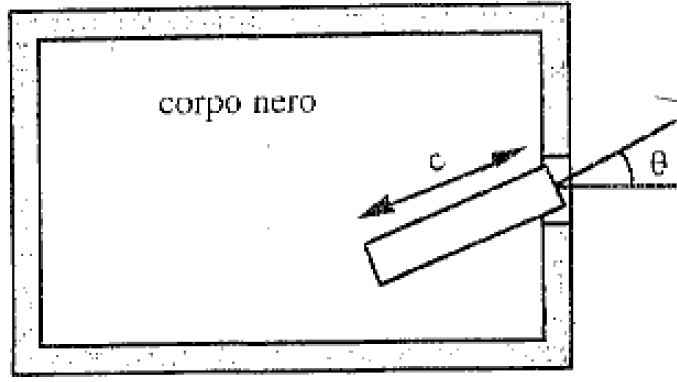
\includegraphics[width=0.4\textwidth]{Immagini/CorpoNero.png}
	\caption{}
	\label{fig:corponero}
	\vspace{-10pt}
\end{wrapfigure}

Si noti che la distribuzione di Planck in funzione della lunghezza d'onda prenderebbe invece la forma:
\begin{equation*}
u_\omega (\omega, T) = \frac{8\pi h c}{\lambda^5} \frac{1}{\exp(hc/\lambda\kt) - 1}
\end{equation*}
essa ha un massimo per:
\begin{equation*}
\lambda_m T \simeq \frac{h c}{k_B} \frac{1}{4.965} \simeq \unit{2897}{\micro\meter  ~\kelvin}
\end{equation*}
Questa relazione è nota come \textit{legge di spostamento di Wien}.
\newline

In realtà ciò che si misura sperimentalmente è la quantità di energia emessa per unità di area e per unità di tempo da una cavità al cui interno si trova la radiazione di corpo nero, cioè l'emissività del corpo nero $ e_\nu (\nu,T) $.

Se $ c\cos \theta $ è il volume occupato dai fotoni che escono sotto l'angolo $ \theta $ nell'unità di tempo da una superficie unitaria (vedi \cref{fig:corponero}), l'emissività è:
\begin{equation*}
e_\nu (\nu,T) = u_\nu \int c \cos \theta \frac{\dd \Omega}{4\pi} = u_\nu \frac{c}{4}
\end{equation*}
e l'energia totale emessa per unità di tempo:
\begin{equation*}
e_\nu (\nu,T) = \int_{0}^{\infty} u_\nu \frac{c}{4} = \frac{2 \pi^5 k_B^4}{15h^3c^2}T^4 = \sigma T^4
\end{equation*}
ed è nota come \textit{legge di Stefan}, mentre $ \sigma $ è la \textit{costante di Stefan-Boltzmann}.

\section{Proprietà geometriche dei cristalli}

Nella precedente sezione si è discusso della capacità termica dei cristalli, ma si è quasi sempre fatto riferimento a teorie di campo medio, e l'unico modello introdotto è quello di cristallo unidimensionale.

Non si è quindi fatto uso di specifiche proprietà geometriche dei cristalli, ma solo del fatto che gli atomi siano spazialmente vincolati al sito che occupano. Si procede dunque in questa sezione a prenderà in esame più in dettaglio quali siano le proprietà geometriche dei cristalli.

\subsection{Reticoli di Bravais}

I cristalli sono caratterizzati da una periodicità discreta, che si realizza in una proprietà fondamentale. Per definirla si consideri un punto $ \textbf{r} $, tutti i punti associati da specifici vettori di traslazione $ \bm{\tau}_n $ sono ad esso equivalenti, cioè indistiguibili.

Il senso di questa affermazione è che dato qualunque punto
\[ \textbf{r}' = \textbf{r} + \bm{\tau}_n \]
tutte le osservabili fisiche assumono lo stesso valore in $ \textbf{r} $ e $ \textbf{r'} $.

La proprietà fondamentale è quindi la seguente: la struttura dei vettori di traslazione introdotti è
\[ \bm{\tau}_{\textbf{n}} = n_1 \bm{\tau}_1 + n_2 \bm{\tau}_2 + n_3 \bm{\tau}_3  \]
dove $ n_1, n_2, n_3 \in \mathbb{N} $ e $ \bm{\tau}_1, \bm{\tau}_2, \bm{\tau}_3 $ sono vettori indipendenti (detti \textit{vettori primitivi}) che definiscono una cella primitiva.

\subsubsection{Proprietà dei reticoli}

L'insieme dei vettori di traslazione $ \bm{\tau}_n $ costituisce il reticolo cristallino, e poiché la somma di due traslazione è ancora una traslazione, e ad ogni traslazione ne corrispone una inversa, tale insieme costituisce un gruppo, chiamato \textit{gruppo delle operazioni di traslazione.}

Un reticolo definito in tal modo è detto \textit{reticolo di Bravais}.
\newline

Una definizione equivalente è che un reticolo di Bravais è un insieme infinito di punti isolati (cioè un insieme discreto) che appare \textit{esattamente} lo stesso da ogni punto dell'insieme\footnote{Questa definizione è meno formale, ma forse più intuitiva. \`E stata inserita per rendre conto della nota sull'orientamento, che può chiarire a livello intuitivo cosa \textit{non} sia un reticolo di Bravais.}

\begin{wrapfigure}{R}{0.3\textwidth}
\vspace{-25pt}
\centering
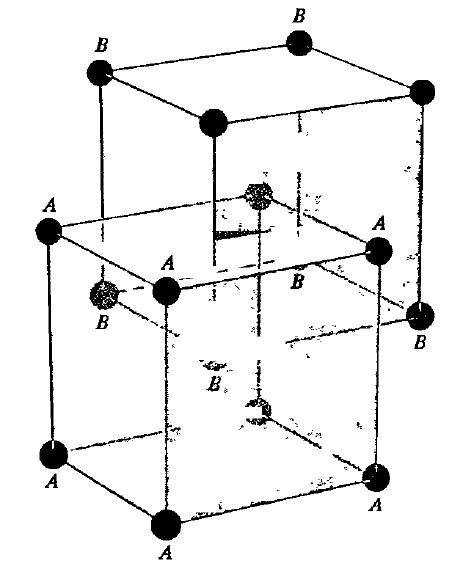
\includegraphics[width=0.3\textwidth]{Immagini/BodyCenteredCubic.png}
\caption{}
\label{fig:bcc}
\vspace{-30pt}
\end{wrapfigure}

La definizione alternativa data è una caratterizzazione intuitiva delle proprietà che definiscon un reticolo di Bravais. \`E però necessario ribadire cosa significhi "esattamente":

\begin{note}[Orientamento]
	Si specifica che, perché i punti siano equivalenti, non solo la disposizione deve essere la stessa (cioè la struttura dei vettori primitivi), ma anche l'orientamento.
	
	Ad esempio la piastrellatura esagonale del piano rispetta il requisito sulla disposizione, ma non quello sull'orientamento.
\end{note}

Per giustificare l'opportunità della definizione alternativa si consideri il seguente esempio.

\begin{es}[Reticolo cubico a corpo centrato]
	\label{es:bcc}
	Nel caso mostrato in \cref{fig:bcc} si ha che gli elementi del reticolo sono i punti appartenenti ai due sistemi di reticoli cubici.
	
	Questo è intuitivo secondo la definizione alternativa, ma non lo è affatto se si tratta di individuare i vettori primitivi: in tal caso appare come se i reticoli fossero due (due reticoli cubici sovrapposti), ma è possibile trovare dei vettori che soddisfino anche questa definizione.
	
	Un esempio di tali vettori sono due spigoli adiacenti di un cubo e il vettore che congiunge il vertice in esame con il centro del cubo. Si verifichi che essi generano entrambi i sottoreticoli cubici.
	
	
	Un altro esempio semplice è il reticolo cubico a facce centrate.
\end{es}

\begin{note}[Reticolo di Bravais]
	Si noti che si è indicato con il termine \textit{reticolo di Bravais} l'insieme dei vettori di traslazione, quindi un sottoinsieme di uno spazio vettoriale.
	
	La denominazione \textit{reticolo di Bravais} viene però usata indifferentemente per indicare tre cose distinte:
	\begin{itemize}
		\item l'insieme dei punti dello spazio (cioè un sottoinsieme di uno spazio affine);
		\item l'insieme dei vettori che li congiunge (cioè un sottoinsieme di uno spazio vettoriale);
		\item l'insieme delle traslazioni che definite dai vettori (cioè un gruppo).
	\end{itemize}
	Insiemisticamente (e intuitivamente) questi tre insiemi sono la stessa cosa, perché in bigezione fra loro, sono distinti solo dalla struttura che li caratterizza.
\end{note}

Si ha inoltre la seguente proprietà per i reticoli:

\begin{defn}[Numero di coordinazione]
Poiché il numero di \textit{primi vicini} non dipende dal punto, a causa della periodicità del reticolo, allora esso è una proprietà del reticolo, ed è chiamato \textit{numero di coordinazione}.
\end{defn}

\subsubsection{Cella primitiva}

Lo stesso reticolo traslazionale può essere ottenuto scegliendo celle primitive diverse, come mostrato in \cref{fig:elcell}. Il nuovo insieme di vettori (quello che definisce la nuova cella) non sarà indipendente dal precedente, ma sono ottenibili l'uno dall'altro con combinazioni lineari a coefficienti interi.

Proprio per quest'ultimo motivo il volume della cella elementare sarà indipendente dalla scelta dei vettori primitivi, infatti il volume di un parallelepipedo è un'applicazione multilineare alternante sui vettori che ne definiscono gli spigoli.
\`E quindi possibile definire la cella elementare proprio come una qualunque cella\footnote{\label{note:cell} Cioè un parallelepipedo definito da vettori del reticolo.} di volume minimo (un altro modo potrebbe essere che non contenga punti del reticolo nella parte interna del suo volume).

\begin{figure}[h]
	\centering
	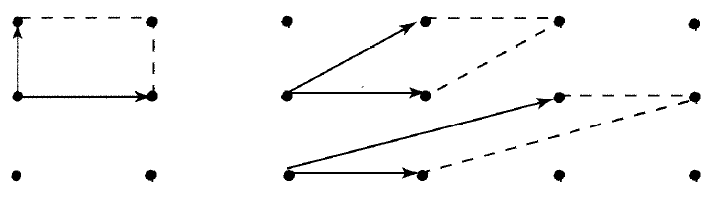
\includegraphics[width=0.6\textwidth]{Immagini/ElementaryCell.png}
	\vspace{-5pt}
	\caption{}
	\label{fig:elcell}
	\vspace{-5pt}
\end{figure}

L'osservazione precedente talvolta viene estesa, per includere nella definizione precedente anche volumi genericim che non sono propriamente "celle" come definite in \cref{note:cell}.

\begin{defn}[Cella primitiva generalizzata]
	La cella primitiva può essere un qualunque volume che se traslato con tutti i vettori del reticolo ha le seguenti proprietà:
	\begin{itemize}
		\item non genera mai due volumi parzialmente sovrapposti\footnote{Totalmente è impossibile per qualunque volume.};
		\item ricopre tutto lo spazio con le copie generate (cioè ogni punto dello spazio apparterrà a una delle copie traslate).
	\end{itemize}
\end{defn}

Dalla definizione precedente risulta che, considerando il caso in cui i punti del reticolo non appartengano al bordo della cella, ogni cella primitiva contiene uno e un solo punto. \`E quindi intuitivo che il volume di una cella sia pari all'inverso della densità dei punti del reticolo di Bravais, per cui anche nel caso generale il volume della cella è indipendente dalla scelta di questa.
\newline

Tornando alla cella primitiva inizialmente considerata, quella definita dai vettori primitivi del reticolo, si ha che essa spesso non rappresenta bene le proprietà di simmetria del reticolo, proprio a causa del numero di modi equivalenti in cui è possibile scegliere i vettori primitivi.
 
Si pensi ad esempio a un reticolo cubico a corpo centrato (vedi \cref{es:bcc}), oppure un reticolo cubico a facce centrate.

Ci sono due soluzioni usate questo tipo di problema:

\subparagraph{Cella unitaria} Si può considerare una cella non primitiva, più grande di una primitiva, che abbia le stesse proprietà di quest'ultima, ma limitando le traslazioni solo a quelle generate da un sottoreticolo del reticolo di Bravais in esame (nel caso cubico a corpo centrato si può considerare la cella cubica e il sottoreticolo cubico).
Essa quindi può essere scelta con le proprietà di simmetria desiderate.

I numeri che specificano le dimensioni della cella unitaria sono detti \textit{costanti reticolari}.

\subparagraph{Cella di Wigner-Seitz} \`E comunque sempre possibile considerare una cella primitiva generalizzata con le proprietà di simmetria del reticolo. Un modo per definire una cella con queste proprietà è quello di associare ogni punto dello spazio al punto del reticolo cui è più vicino\footnote{\label{note:wigseitz} I punti equidistanti da due o più elementi del reticolo si possono anche scartare, essi costituiscono un insieme a misura nulla, di dimensione più bassa rispetto alla dimensione del reticolo, a causa dei vincoli imposti dalla relazione di equidistanza.}.

L'insieme di tutti i punti così associati ad un elemento del reticolo costituisce una cella primitiva, detta \textit{cella di Wigner-Seitz}.
Poiché non c'è nessun riferimento in questa definizione ai vettori primitivi del reticolo questa cella avrà le stesse proprietà di simmetria del reticolo di Bravais.

\begin{oss}[Costruzione geometrica]
	La cella di Wigner-Seitz associata a un dato elemento del reticolo di Bravais può essere costruita connettendo tale elemento ai suoi primi vicini, e bisecando i segmenti congiungenti con iperpiani perpendicolari ad essi (rette per reticoli in 2D, piani in 3D, \dots).
	La cella è ottenuta considerando tali iperpiani come bordi di essa.
	
	I punti degli iperpiani sono proprio quelli che realizzano la relazione di equidistanza citata in \cref{note:wigseitz}. 
\end{oss}

\subsubsection{Reticoli con una base} 

Un cristallo è spesso organizzato in modo più complesso di quello che può essere descritto dal solo reticolo di Bravais associato. 
Si può infatti considerare un cristallo in cui gli elementi del reticolo non siano semplici atomi, ma molecole, o altre strutture.

In questo caso si parla di \textit{struttura cristallina}, cioè un reticolo di Bravais i cui elementi sono strutture fisiche non elementari.

Più in generale si parla di \textit{reticoli con una base}, in cui al singolo elemento del reticolo di Bravais non è necessariamente associata un unica struttura fisica, ma anche una struttura geometrica costituita da più unità fisiche separate.

Quest'ultimo caso è esemplificato in \cref{fig:honey}, dove è mostrata una piastrellatura esagonale del piano.

\begin{figure}[h]
	\centering
	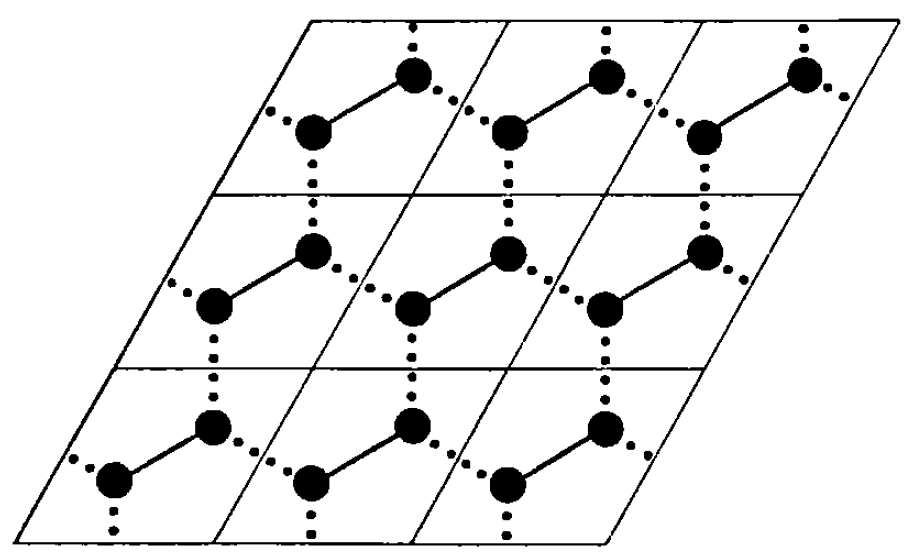
\includegraphics[width=0.6\textwidth]{Immagini/HoneycombLattice.png}
	\vspace{-5pt}
	\caption{}
	\label{fig:honey}
	\vspace{-5pt}
\end{figure}

Anche nel caso di reticoli di Bravais puri è possibile considerarli come reticoli con una base, ad esempio nel caso del reticolo cubico a corpo centrato, scegliendo come cella una cella unitaria non primitiva, e fissando gli elementi interni alla cella come \textit{base}.

%\paragraph{Gruppi di simmetria} \`E possibile ottenere tutti i gruppi di simmetria realizzabili da un cristallo tridimensionale: essi sono $ 230 $ (ottenuti da $ 14 $ reticoli di traslazione e $ 32 $ gruppi puntuali, di cui $ 7 $ oloedrici).
%Non si vuole studiare in dettaglio questa affermazione, né è importante chiarire il significato dei termini usati, ma è importante sapere che i gruppi cristallini sono completamente classificati e in numero limitato.

\subsection{Reticolo reciproco}

\begin{defn}[Reticolo reciproco]
	Si definisce reticolo reciproco di un reticolo di Bravais l'insieme dei vettori $ \textbf{K} $ che definiscono onde piane con la periodicità del reticolo di Bravais associato. Cioè:
	\[ e^{i\textbf{K}\cdot (\textbf{r} + \textbf{R})} = e^{i\textbf{K}\cdot \textbf{r}} \]
	per ogni $ R $ appartenente al reticolo di Bravais.
	
	O, più semplicemente, $ K $ appartiene al reticolo reciproco se:
	\[ e^{i\textbf{K}\cdot \textbf{R}} = 1 \]
	per ogni $ R $ appartenente al reticolo di Bravais.
\end{defn}

Il reticolo di Bravais associato al reticolo reciproco è detto di solito \textit{reticolo diretto}.

\subsubsection{Reticolo di Bravais}

Anche il reticolo reciproco è un reticolo di Bravais, infatti se due vettori appartengono al reticolo reciproco anche qualunque loro combinazione lineare a coefficienti interi appartiene al reticolo reciproco.

Inoltre è facile trovare i vettori primitivi del reticolo reciproco tridimensionale, essi saranno:
\begin{align*}
\textbf{b}_1 = 2\pi \frac{\textbf{a}_2 \times \textbf{a}_3}{\textbf{a}_1 \cdot (\textbf{a}_2 \times a_3)}\\
\textbf{b}_2 = 2\pi \frac{\textbf{a}_3 \times \textbf{a}_1}{\textbf{a}_1 \cdot (\textbf{a}_2 \times a_3)}\\
\textbf{b}_3 = 2\pi \frac{\textbf{a}_1 \times \textbf{a}_2}{\textbf{a}_1 \cdot (\textbf{a}_2 \times a_3)}
\end{align*}
dove $ \textbf{b}_i $ sono i vettori primitivi del reticolo reciproco e $ \textbf{a}_j $ quelli del reticolo diretto.
Per provarlo è sufficiente verificare che sia soddisfatta:
\[ \textbf{b}_i \cdot \textbf{a}_j = 2\pi \delta_{ij} \]
dove $ \delta_{ij} $ è la delta di Kronecker.

Per cui ogni vettore del reticolo reciproco può essere scritto come:
\[ \textbf{k} = k_1 \textbf{b}_1 + k_2 \textbf{b}_2 + k_3 \textbf{b}_3\]
e ogni elemento del reticolo diretto:
\[ \textbf{R} = n_1 \textbf{a}_1 + n_2 \textbf{a}_2 + n_3 \textbf{a}_3\]
e dalla relazione $ e^{i\textbf{k}\cdot\textbf{R}} = 1 $ deriva che i $ k_i $ devono essere interi, poiché gli $ n_j $ lo sono.

\paragraph{Il reciproco del reciproco} Poiché il reticolo reciproco è anch'esso un reticolo di Bravais si può esaminare chi sia il \textit{suo} reciproco.
Esso risulta essere il reticolo diretto, e un modo per provarlo è applicare due volte la formula per i vettori primitivi.

Un modo più facile è accorgersi che la condizione che devono soddisfare i vettori del reciproco del reciproco è $ e^{i\textbf{K}\cdot\textbf{G}} = 1$, ma poiché tale condizione è simmetrica in $ \textbf{G},\textbf{K} $ è soddisfatta dagli elementi del reticolo diretto. Non ci possono essere ulteriori elementi non appartenenti al reticolo diretto per la definizione dei $ \textbf{b}_i $, se infatti si associano agli $ \textbf{a}_j $ coefficienti non interi il prodotto scalare sarà non intero per alcuni vettori del reciproco.

\begin{es}
	Il reticolo reciproco di un reticolo cubico semplice è ancora un reticolo cubico semplice.
	
	I reticoli cubici a facce centrate e a corpo centrato sono uno il reciproco dell'altro.
\end{es}

\paragraph{Volume della cella} Il volume della cella primitiva del reticolo reciproco si trova facilmente a partire dalle espressioni esplicite per i $ \textbf{b}_i $, esso è $ (2\pi)^3/v $, dove $ v $ è il volume della cella primitiva del reticolo diretto.


\subsection{Zone di Brillouin}

\subsection{Diffrazione dei raggi X}

\section{Hamiltoniana dei Cristalli}

\subsection{Approssimazione di Born-Oppenheimer}

\subsection{Hartree-Fock}

\section{Il teorema di Bloch}

\subsection{Il concetto di banda}